%%=============================================================================
%% PROOF-OF-CONCEPT
%%=============================================================================

\chapter{\IfLanguageName{dutch}{Werking huidig systeem}{Operation of the current system}}%
\label{ch:current system}

\section{Inleiding}
\label{sec:inleiding_currsys}
Dit hoofdstuk zal de werking van het huidige systeem om coolgen applicaties te ontwikkelen van ArcelorMittal Gent toelichten en visualiseren. De stappen die in het huidige systeem aanwezig zijn zullen ook terug te vinden zijn in het nieuwe systeem met behulp van een pipeline en IBM DBB. Het is uiterst noodzakelijk om kennis te hebben van het huidige systeem alvorens een nieuw systeem kan gemaakt/geïmplementeerd worden. Dit komt doordat het systeem dat momenteel gebruikt uitermate veel is gepersonaliseerd door ArcelorMittal Gent om aan hun eisen en gebruiken te voldoen. 

\section{Compileren}
\label{sec:compileren}
De huidige geïnstalleerde versie van de Cobol compiler binnen ArcelorMittal Gent is versie 6.20, deze versie van Cobol is geïntroduceerd in 2017 op 8 september en heeft geen support meer vanaf 30 september 2024.
\\ \\
De JCL die uitgevoerd wordt wanneer men een compilatie van een programma wil uitvoeren wordt opgeroepen via een product van Rocket software namelijk MSP (Manager Products). Dit product zorgt ervoor dat een ontwikkelaar kan meegeven welk programma hij/zij wil compileren en in welke omgeving die dat wil doen, dit kan bijvoorbeeld productie of ontwikkeling zijn. Dat product zorgt er dan voor dat de JCL voor de compile uit te voeren wordt gestart met de juiste parameters en de juiste libraries die moeten meegegeven worden tijdens de compilatie zoals de SYSLIB en SYSIN DD's.
\\ \\
Heel belangrijk binnen het huidig systeem is het gebruik van meta-data, hierdoor weet in dit geval MSP welke parameters die moet aanvoeren aan de compiler, welke libraries die moet alloceren en of er extra zaken moeten gestart worden zoals een Db2 package bind of Db2 plan bind. Deze meta-data is dan ook een van de eerste zaken dat gecontroleerd wordt als men een compilatie wil starten. Indien er geen meta-data te vinden is dan zal de compile geannuleerd worden. 
\\ \\
Deze meta-data bevat onder andere informatie over de afdeling waar het gemaakt is, de programmeur van de applicatie, wat voor soort applicatie het is. Zo heb je 3 verschillende soorten programma's binnen ArcelorMittal Gent, je hebt de main programma's, die kunnen ofwel volledig onafhankelijk draaien of ze roepen sub programma's op. Deze main applicaties kunnen zelf niet opgeroepen worden door andere applicaties. Als laatste zijn er ook nog 2 soorten sub programma's, de fsub en de sub. In theorie is er niet veel verschil buiten de manier waarop ze opgeroepen kunnen worden. Zo wordt een sub statisch gebindt aan een programma dat hem oproept en een fsub wordt dynamisch opgeroepen tijdens de run time. Naast die 3 soorten van applicaties is er ook nog het feit of er gebruik gemaakt wordt van subsystemen zoals IMS, Db2 of MQ. Indien hiervan gebruik gemaakt wordt dan kan de ontwikkelaar ook deze zaken aanduiden binnen het meta-data scherm van zijn/haar applicatie. 
\\ \\
Eenmaal alle meta-data aanwezig is zal MSP met behulp van skeletons de juiste JCL opmaken om die applicatie te compileren met de juiste libraries en parameters. De compile parameters zijn heel gelijkaardig voor alle soorten programma's maar kunnen toch nog ergens licht afwijken. Zoals wanneer er gebruik gemaakt wordt van een subsysteem zoals IMS of Db2.
\\ \\

\section{Bind}
\label{sec:bind}
Er wordt gebruik gemaakt van de IEWL Binder voor z/OS 2.5 om de applicaties van ArcelorMittal te binden. Het belangrijkste verschil tussen een programma dat gebind is met IEWL en een dat gelinkedit is, is het feit dat bij de linkedit een groot uitvoerbaar bestand gemaakt wordt van de verschillende objectbestanden van het hoofdprogramma, de subprogramma's en de subroutines die opgeroepen worden. Hierdoor is het programma dat gelinkedit wordt statisch aangemaakt, dit wil zeggen dat indien er een sub programma verandert er dus een nieuwe linkedit moet gebeuren van alle progamma's die dat sub programma gebruiken. Met een binder kan je dynamisch een programma aan een ander programma koppelen/binden, op die manier is het zo dat een sub programma opgeroepen wordt op run time en niet tijdens de compile. Hierdoor hoeft er geen herlink meer te gebeuren van de applicaties die dat programma gebruiken. 
\\ \\
Er zijn net zoals bij de compilatie ook parameters die meegegeven worden aan de binder om op de juiste manier de programma's te kunnen binden. In tegenstelling als bij de compilatie moet er niet voor elk soort programma (main, Db2, IMS, sub, ...) een aparte parameter lijst gemaakt worden. De parameters zijn hetzelfde voor main- en fsub programma's aangezien die worden opgeslagen als DLL, voor de sub programma's is er een andere parameter lijst die ervoor zorgt dat de sub geen DLL wordt maar statisch blijft. Hierdoor zullen main- en fsub programma's wel dynamisch opgeroepen kunnen worden tijdens run time en zal er voor sub programma's opnieuw met herlink en hercompile moeten gewerkt worden. 
\\ \\ 
De binder wordt net zoals de compiler opgeroepen door het product MSP, het gaat op dezelfde manier te werk als bij de compile en maakt gebruik van een applicatie zijn meta-data om zo de juiste libraries en parameters mee te geven.

\chapter{Proof Of Concept}
\label{ch:poc}

\section{Inleiding}
\label{sec:inleiding_poc}
Het hoofdstuk van de Proof Of Concept zal gaan over welke stappen en producten er allemaal nodig waren om de proefopstelling succesvol te laten werken. Deze stappen zullen overeenkomen met die van het huidige systeem besproken in het vorige hoofdstuk.
\\ \\

\section{Installatie \& configuratie IBM DBB}
\label{sec:installdbb}
De eerste stap in het opzetten van de proefopstelling is om de IBM DBB installatie af te ronden en de configuratie te starten. De installatie op de mainframe van ArcelorMittal werd gedaan door een bedrijf genaamd NRB, zij zijn verantwoordelijk voor installatie van software op de mainframe van ArcelorMittal Gent. 
\\ \\
Aangezien IBM DBB al geïnstalleerd is voor deze Proof Of Concept kan er direct begonnen worden aan de configuratie van de bestanden die gebruikt worden door het product DBB. Deze bestanden zijn onder andere properties bestanden die ervoor zorgen dat bepaalde zaken zoals de binder en compiler worden gedeclareerd. Deze zijn niet standaard meegeleverd en moeten afgehaald worden vanaf een git repository namelijk de dbb-zappbuild git repository van IBM. 
\\ \\
\subsection{Installatie dbb-zappbuild}
Die repository kan rechtstreeks gecloned worden of via file transfer kunnen die ook op de juiste plaats in de USS belanden. De aanbevolen plaats om die repository te stockeren is in de hoofdfolder van DBB, dat ziet eruit zoals /dbb/dbb-zappbuild.
\\ \\
\subsection{Configuratie dbb-zappbuild}
Nu dat de dbb-zappbuild repository aanwezig is op de USS kan er begonnen worden aan de configuratie van DBB. Deze configuratie op de USS bestaat hoofdzakelijk uit properties en .groovy bestanden. De properties bestanden zijn te vinden in de folder build-conf en zijn ook de eerste die moeten veranderd of ingevuld worden. Verder zijn er de .groovy bestanden die voor de verwerking van die properties zorgen, dit is in een hoofdprogramma (build.groovy), language specifieke programma's zoals Cobol.groovy en utility programma's zoals BuildUtilities.groovy.
\\ \\
Deze bestanden hebben elk hun eigen taken en nut in de werking van het systeem, zo zijn de properties bestanden noodzakelijk om datasets en PDS'en mee te geven om zo de juiste binder, compiler, load libraries en dergelijke te hebben. De taak van een language specifiek groovy programma zoals Cobol.groovy is om de compilatie en bind van een programma dat in die taal geschreven is uit te voeren. Dit kan heel erg verschillen tussen talen door, zo is de compilatie van een PL/I programma een stuk anders dan de compilatie van een Cobol programma. De zaken die nodig zijn om die compilatie en bind goed uit te voeren kunnen gevonden worden in zo'n language specifiek groovy programma. Deze language specifieke programma's gebruiken heel vaak utility programma's om zaken die hetzelfde zijn in elke taal te bundelen zo is er een BindUtilities.groovy dat een DB2 package bind en/of plan bind kan doen. Dit is onafhankelijk van welke taal je gebruikt en kan dus in zo'n utility programma. Als laatste om de cyclus te vervolledigen is er de build.groovy, dit is het hoofdprogramma dat alle andere programma's op de juiste moment oproept.
\\ \\
\begin{figure}[h]
\begin{tabularx}{1\textwidth} { 
        | >{\centering\arraybackslash}X 
        | >{\centering\arraybackslash}X 
        | >{\centering\arraybackslash}X 
        | >{\centering\arraybackslash}X  | }
    \hline
    Properties bestanden & 
    Language groovy bestanden & 
    Utility groovy bestanden & 
    build.groovy \\
    \hline
    Dataset en PDS declaratie & 
    Oproepen van utilities en language specifieke werking bepalen & 
    Werking van language onafhankelijke procedures bepalen & 
    Oproepen van de juiste groovy sub programma's \\ 
    \hline
\end{tabularx}
\caption{Soorten bestanden en hun taak}
\label{tab:soorten bestanden}
\end{figure}

\subsubsection{Properties bestanden}
Er zijn in totaal 16 properties bestanden waarin aanpassingen moeten aangebracht worden deze zijn onderverdeeld in de verschillende talen en gebruiken. Zo zijn er properties bestanden voor Cobol, PL/I, PSB, ACB en nog een aantal anderen. Er is ook een datasets.properties bestand waarin veel algemene PDS'en en datasets worden gedeclareerd. Zo kan je bijvoorbeeld de z/OS macro library, Cobol compiler, PL/I compiler en DB2 load library vinden en declareren in de datasets.properties. 
\\ \\
In de build.properties zit er vooral algemene instellingen en dus geen datasets, zo kan je aanduiden welke properties bestanden ingeladen kunnen worden als het systeem geactiveerd word. Deze zit net zoals de datasets.properties en de overige taal- en gebruiksspecifieke properties bestanden in de build-conf folder die te vinden is binnen de dbb-zappbuild map. 
\\ \\
De taal specifieke properties worden aangepast in onder andere Cobol.properties en de PLI.properties bestanden. Hierin worden onder andere instellingen zoals load libraries, vereiste properties en compiler opties meegegeven die algemeen gelden voor alle programma's van die taal. De volledige properties bestanden zijn te vinden in appendix \ref{ch:appropsbuild}.
\\ \\
\subsubsection{Language groovy bestanden}
De language groovy bestanden zorgen ervoor dat de programma's van die taal succesvol gecompileerd en gebind kunnen worden. Naast de compile en bind wordt er ook gezorgd dat de load module van de applicatie op de juiste plaats beland, dat er een DB2 package bind en/of plan bind uitgevoerd wordt indien nodig. Zo wordt ervoor gezorgd dat het programma niet alleen goed wordt gecompileerd en gebind maar ook uitvoerbaar is op het mainframe van ArcelorMittal Gent. Binnen dit onderzoek is het enigste language groovy programma de Cobol.groovy, de belangrijkste aangepaste methodes zijn te vinden in appendix \ref{ch:aplangroovy}.
\\ \\
\subsubsection{Utility groovy bestanden}
De utility groovy programma's worden door zowel de language groovy bestanden als de build.groovy opgeroepen om language onafhankelijke procedures op te roepen. Zo is er een groovy utility programma dat ervoor zorgt dat onder andere de build lijst wordt aangemaakt, meta data wordt ingevuld, logicalfiles worden aangemaakt en ervoor zorgt dat datasets kunnen aangemaakt worden. Dit is maar een kleine opsomming van de mogelijkheden van de BuildUtility.groovy, hiernaast zijn er nog 7 andere groovy utility programma's. De enigste programma's die aangepast zijn in het kader van het onderzoek zijn BuildUtilities.groovy en BindUtilities.groovy, de belangrijkste aangepaste methodes zijn te vinden in appendix \ref{ch:aputilgroovy}. 
\\ \\
\subsubsection{build.groovy}
Dit groovy programma roept andere programma's op zoals de utility programma's en de language specifieke programma's. Er wordt een build lijst gemaakt op basis van de rangschikking die meegegeven wordt binnen de properties van de build. Er worden dus groovy bestanden aangeroepen en de properties worden ingeladen zodat die gebruikt kunnen worden door de build.groovy en de andere groovy programma's. 
\\ \\
Hieronder een opsomming van alle bestanden en programma's die ervoor zorgen dat DBB de programma's en bestanden kan compileren, binden en opslaan in een z/OS omgeving.
\begin{multicols}{2}
    \begin{itemize}
        \item \textbf{Properties bestanden}
        \begin{itemize}
            \item ACBgen.properties
            \item Assembler.properties
            \item build.properties
            \item Cobol.properties
            \item datasets.properties
            \item DBDgen.properties
            \item defaultzAppBuildConf.properties
            \item dependencyReport.properties
            \item LinkEdit.properties
            \item MFS.properties
            \item PLI.properties
            \item PSBgen.properties
            \item Transfer.properties
            \item ZunitConfig.properties
        \end{itemize}
        
        \item \textbf{Language groovy bestanden}
        \begin{itemize}
            \item Assembler.groovy
            \item Cobol.groovy
            \item DBDgen.groovy
            \item LinkEdit.groovy
            \item MFS.groovy
            \item PLI.groovy
            \item PSBgen.groovy
            \item Transfer.groovy
            \item ZunitConfig.groovy
        \end{itemize}
        
        \item \textbf{Utility groovy bestanden}
        \begin{itemize}
            \item BindUtilities.groovy
            \item BuildUtilities.groovy
            \item BuildReportUtilities.groovy
            \item DependencyScannerUtilities.groovy
            \item FilePropUtilities.groovy
            \item GitUtilities.groovy
            \item ImpactUtilities.groovy
            \item ReportingUtilities.groovy
        \end{itemize}
        
        \item \textbf{build.groovy}
    \end{itemize}
\end{multicols}
\\ \\
\subsection{Configuratie DBB buiten USS}
Naast de configuratie van DBB in de zapp-build op USS is er ook een configuratie die in elke repository meegegeven moet worden bij het starten van DBB. Dat zijn properties bestanden die in de repository meegeleverd moeten worden om de compilatie en bind in goed uit te voeren. Deze properties bestanden hebben altijd een application.properties en een file.properties, hierin wordt er onder meer een build lijst rangschikking meegegeven om te beslissen in welke orde programma's zullen gecompileerd worden. Naast de application- en file.properties moet er ook per taal een properties bestand meegegeven worden met extra instellingen die toegevoegd worden aan de al beschikbare instellingen die in de properties op USS zijn gedeclareerd. Zo moet er bij de verwerking van een Cobol programma de file-, application- en Cobol.properties bestanden aanwezig zijn binnen de repository. 
\\ \\
Er zijn in totaal voor ArcelorMittal 10 properties bestanden die meegegeven kunnen worden binnen een repository. Deze worden hieronder opgesomd.
\begin{multicols}{2}
    \begin{itemize}
        \item application.properties
        \item Assembler.properties
        \item Cobol.properties
        \item file.properties
        \item languageConfigurationMapping
        \item LinkEdit.properties
        \item PLI.properties
        \item reports.properties
        \item Transfer.properties
        \item ZunitConfig.properties
    \end{itemize}
\end{multicols}
\\ \\
Naast de properties bestanden is er nog een .gitattributes bestand dat heel belangrijk is in verband met het omzetten van de encodering van z/OS naar git en omgekeerd. Op de mainframe van ArcelorMittal Gent wordt er gebruik gemaakt van de EBCIDIC IBM 1148 encodering en die is niet standaard ondersteund door git. Daardoor moet er in een .gitattributes bestand aangegeven worden dat de input in die EBCIDIC encodering staat en dus nog moet omgezet worden naar UTF-8. De properties bestanden en .gitattributes die gebruikt worden binnen de repository van dit onderzoek zijn volledig aangepast terug te vinden in appendix \ref{ch:appropappli}. 

\pagebreak

\section{Opzetten pipeline Azure DevOps}
Om de compilatie en bind van programma's te voltooien wordt er gebruik gemaakt van pipelines en pipeline software om dat proces te starten. In dit onderzoek zal er gebruik gemaakt worden van Azure Pipelines, een product uit de Azure DevOps suite. De reden dat er gebruik gemaakt wordt van Azure Pipelines en niet van een andere pipeline software zoals Jenkins is door het feit dat ArcelorMittal Gent al een licentie had voor Azure DevOps. Zo wordt de software stack van ArcelorMittal niet onnodig uitgebreid. 

\subsection{Azure DevOps workflow}
Voordat er gestart kan worden moet er bekeken worden welke workflow er gebruikt zal worden binnen de pipeline en Azure DevOps. De workflow die gebruikt wordt in dit onderzoek is heel standaard en zal gaan van een desktop met IDz of Visual Studio Code naar het eindstation z/OS. Dit gaat als volgt te werk, er wordt begonnen vanaf niks dus er is nog geen enkele repository die op de desktop staat. 
\\ \\
De eerste stap is dus om een repository te clonen naar een lokale map, dit kan rechtstreeks vanuit IDz of Visual Studio Code. Dan wordt die repository lokaal aangepast door bijvoorbeeld een nieuwe branch toe te voegen, nieuwe commits of nieuwe code. Als de repository klaar is om doorgestuurd te worden naar z/OS dan wordt er via een ``git push'' een signaal verstuurd naar de centrale repository en die zal dan op zijn beurt een of meerdere pipeline jobs lanceren die uitgevoerd worden door een agent die ofwel op Linux of Windows draait. Die pipeline job zal de repository gaan clonen op z/OS, daarna wordt die repository met behulp van IBM DBB gebuild en de bekomen load modules en source files worden daarna op z/OS opgeslagen. De visuele weergave van deze workflow is te vinden op figuur \ref{fig:azure devops flow}.
\begin{figure}[h]
    \centering
    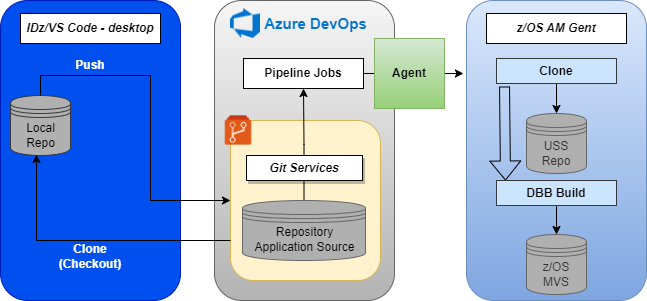
\includegraphics[scale=0.65]{AzureDevOps_Flow}
    \caption{Azure DevOps workflow}
    \label{fig:azure devops flow}
\end{figure}

\subsection{Opzetten van een organisatie, agent pool en agent in Azure DevOps}
Er wordt gewerkt binnen Azure DevOps met organisaties zo kan er op een makkelijke en overzichtelijke manier gescheiden gewerkt worden van andere takken en/of teams binnen een bedrijf. Voordat er kan begonnen worden aan het proces om een organisatie en agent op te zetten moet er toegang zijn tot Azure DevOps. Dit wil zeggen dat er een geregistreerd account ter beschikking moet zijn met de nodige privileges om een organisatie te mogen aanmaken. Indien dat ter beschikking is zouden er geen problemen mogen zijn met het opzetten van een organisatie en agent. 
\begin{enumerate}
    \item Inloggen op Azure DevOps.
    \item Aanmaken van een full acces \textbf{P}ersonal \textbf{A}cces \textbf{T}okens.
    \item Creëer een nieuwe organisatie.
    \item Toevoegen van een self hosted agent pool.
    \item Maken van een nieuwe agent op een Windows machine.
    \item Configureren van de Windows agent.
    \item Starten van de agent. 
\end{enumerate}
\autocite{Microsoft2024a}
\autocite{Microsoft2024b}
\autocite{Microsoft2024c}
\\ \\
Het nut van een agent pool en agents is om de pipelines uit te laten voeren. Elke agent kan 1 pipeline uitvoeren. Indien er twee pipelines zijn die uitgevoerd moeten worden, zal er een van de twee in een queue geplaatst worden totdat de agent terug beschikbaar is. Binnen een agent pool kunnen er meerdere agents geïnstalleerd zijn. Hierdoor is het mogelijk om meerdere pipelines tegelijk te laten uitvoeren binnen dezelfde agent pool. 
\\ \\
Het is mogelijk om restricties te plaatsen op agents of agent pools in verband met welke pipelines ze mogen/kunnen uitvoeren. Zo kan er een eigen agent pool zijn voor bijvoorbeeld een migratie pipeline en een voor de compilatie/bind van programma's. 

\subsection{Azure DevOps project en connectie met de mainframe}
Binnen een organisaties kunnen er meerdere projecten aangemaakt worden, zo kan er op een overzichtelijke manier gewerkt worden binnen Azure DevOps. Elk project heeft zijn eigen resources, zo kunnen er bijvoorbeeld meerdere Azure Repo's en Azure Pipelines aangemaakt worden per project. 
\\ \\
Naast de resources die al aan bod gekomen zijn is er ook de mogelijkheid om service connecties te leggen, in deze proof of concept werd dat gedaan naar de mainframe van ArcelorMittal Gent. Dit gebeurt binnen de project instellingen en dan service connections, op die manier kan er een SSH connectie gemaakt worden met een mainframe of bij uitbreiding een andere server/computer waarmee verbinding wenst gemaakt te worden. 
\\ \\
In het geval van dit onderzoek wordt er gebruik gemaakt van één project waarin geconnecteerd wordt naar de mainframe van ArcelorMittal Gent met behulp van de SSH service connectie. Voor de SSH verbinding moeten de juiste waarden ingevuld worden zoals host name en poort nummer. De authenticatie gebeurt via een RACF user en paswoord, zo is bij het onderzoek gebruik gemaakt van een persoonlijke user. Indien het paswoord van die user verandert zal ook de service connectie moeten aangepast worden naar het nieuwe paswoord.

\subsection{Azure Repo toewijzen aan een project}
Voordat er kan gewerkt worden op een remote repository moet er eerst een aangemaakt worden, dit gebeurt via het online portaal van Azure DevOps binnen het project waarin de repo aangemaakt dient te worden. 
\\ \\ 
Er kan gekozen worden om een nieuwe repo aan te maken of om te starten van een bestaande repository via een import, dit onderzoek zal starten vanaf een lege repository. 

\subsection{Azure Pipeline toewijzen aan een project}
De verbinding van de repository naar de mainframe wordt behandeld door een pipeline. Dit kan letterlijk gezien worden zoals de naam het aangeeft, het is een pijplijn waardoor allerhande informatie en bestanden wordt doorgegeven aan de repository, de user en de mainframe. 
\\ \\
Een pipeline wordt aangemaakt binnen een project en werkt door middel van bash scripts, de bash scripts die nodig zijn voor het werken met IBM DBB worden aangeboden door IBM in een document genaamd \enquote{Azure DevOps and IBM Dependency Based Build Integration}, hierin staan de voorgestelde scripts in vermeld. 
\\ \\
Het is aangeraden om te beginnen met een basisscript dat bijvoorbeeld de mappenstructuur toont of de aangemelde user alvorens te springen op de DBB scripts. De scripts van IBM werden aangepast naar de eisen van ArcelorMittal en wijken dus licht af ten opzichte van de originele scripts. Zowel de aangepaste als de originele scripts zijn te vinden in appendix \ref{ch:apbashpipe}.

\subsection{Testen werking pipeline}
Om er zeker van te zijn dat er over kan gegaan worden naar het gebruik van de IBM DBB bash scripts moet er zekerheid zijn dat de pipeline de goeie connectie maakt naar de mainframe en moet er ook gecloned kunnen worden binnen de USS. Met andere woorden Git moet daar goed geïnstalleerd zijn. Deze zaken kunnen makkelijk getest worden, het eerste wat getest is in dit onderzoek is of er wel degelijk een connectie was. Dat werd getest door een pipeline met het commando \enquote{whoami}, als dat de juiste user weergaf zoals opgegeven bij het aanmaken van de service connectie dan was er geen probleem. Indien die niet werd weergegeven dan is er iets fout gelopen bij de service connectie en moet die stap opnieuw gedaan/bekeken worden. 
\\ \\
Als er vastgesteld is dat er een connectie kan gemaakt worden met de mainframe is er in dit onderzoek gekeken naar Git op de USS. Daarvoor zijn er twee stappen namelijk zorgen dat Git geïnstalleerd is op de user die gebruikt wordt voor de service connectie en zorgen dat die user ook een Azure Repo kan clonen. 
\\ \\
Om te zien of Git geïnstalleerd is op de user zijn USS wordt het \enquote{git --version} commando gebruikt. Als dat een versie van git weergeeft wil dat zeggen dat Git geïnstalleerd is op die user zijn USS, indien er een boodsschap weergegeven wordt dat het commando niet gevonden werd dan is Git nog niet (goed) geïnstalleerd. 
\\ \\ 
Nadat vastgesteld is dat Git goed is geïnstalleerd kan de configuratie voor het clonen beginnen. De clone zal gebeuren aan de hand van een Personal Acces Token (PAT), met PAT kan er connectie gemaakt worden via HTTPS en niet via SSH. Eerste stap in dit proces is om een PAT aan te maken, dit kan via het Azure Repos dashboard door op de knop clone te klikken en dan git credentials aan te laten maken. Het paswoord dat gecreëerd wordt is uitermate belangrijk want deze wordt nergens bijgehouden door Azure DevOps om later terug op te vragen. Dat paswoord moet dan enkel nog omgezet worden naar een Base 64 encoding, dit kan via powershell op windows via de volgende commando's:
\begin{enumerate}
    \item \$MyPat='gekopieerd paswoord'
    \item \$B64Pat=[Convert]::ToBase64String([System.Text.Encoding]::UTF8.GetBytes(\textquotedblleft`:\$MyPat\textquotedblright))
    \item echo \$B64Pat
\end{enumerate}
Na deze commando's verkrijg je de Base 64 geëncodeerde versie van het paswoord en diegene die gebruikt dient te worden door Git op het USS. Om de clone succesvol uit te voeren is het nodig dat het Base 64 geëncodeerd paswoord wordt opgeslagen in de git config. Dit kan ingesteld worden door het \enquote{git config --global http.extraheader \textquotedblright Authorization: Basic GEKOPIEERD B64 PASWOORD\textquotedblleft} commando in te geven binnen een terminal zoals dat kan op IDz. Hierna kan het git clone commando uitgevoerd worden zonder problemen. 
\\ \\
Als beide testen vlekkeloos verlopen zijn dan pas kan er overgegaan worden op de IBM DBB bash scripts. 

\subsection{Pipeline taken, variabelen, opties \& triggers}
Het gebruik van de IBM DBB bash scripts kan enkel en alleen als er ook een aantal variabelen gedefinieerd zijn. Zo moet er een nieuwe SSH taak toegevoegd worden aan de pipeline met daarin het commando om het bash script te starten en daarna de script parameters. In het kader van dit onderzoek ziet het commando voor het AzRocketGit-init.sh script eruit als \enquote{./AzRocketGit-init.sh \$(MyRepo) \$(MyWorkDir) \$(Build.SourceBranch)} en het AzDBB-build.sh script ziet eruit als \enquote{./AzDBB-build.sh \$(MyWorkDir) \$(MyRepo) \$(MyApp) --impactBuild}.
\\ \\
De taken gebruiken variabelen, op die manier kan een pipeline bij meerdere repositories ingezet worden. Azure Pipeline komt inclusief een hele hoop standaard variabelen maar een aantal zijn zelf moeten aangemaakt worden voor dit onderzoek. Diegene die rechtstreeks gebruikt worden in de taken zijn de volgende. 
\begin{figure}[h]
    \begin{tabularx}{1\textwidth} { 
            | >{\centering\arraybackslash}X 
            | >{\centering\arraybackslash}X 
            | >{\centering\arraybackslash}X  | }
        \hline
        \textbf{Naam} & 
        \textbf{Waarde} & 
        \textbf{Uitleg} \\
        \hline
        git &
        Pad naar rocket Git client op USS. &
        Zorgt ervoor dat de Git client gevonden wordt door de pipeline \\ 
        \hline
        MyApp &
        source &
        De plaats binnen de repository waar het script de source code kan vinden. \\ 
        \hline
        MyRepo &
        \$(Build.Repository.Uri) &
        De link van de repository. \\ 
        \hline
        MyWorkDir &
        \$HOME/Azure-WorkSpace/ \$(System.TeamProject)-\$(Build.buildid) &
        De plaats waar de repository gekloond wordt en de logs aangemaakt. \\ 
        \hline
        system.teamProject &
        Projectnaam &
        De projectnaam waarin de pipeline is gemaakt. \\ 
        \hline
    \end{tabularx}
    \caption{Pipeline variabelen en hun taak}
    \label{tab:soorten pipeline variabelen}
\end{figure}
\\ \\
De opties zijn voor dit onderzoek op de standaardwaarden gehouden, bij de pipeline opties zit onder andere hoelang een pipeline maximaal mag duren en indien die gecanceld wordt hoelang die maximum mag nemen om de job te cancelen.  
\\ \\
Als laatste zijn er nog triggers die kunnen ingesteld worden voor de pipeline. Hiermee kan continuous integration geactiveerd worden voor bepaald branches of net gedeactiveerd. Zo kan er voor de branch develop continuous integration geactiveerd zijn en voor de main branch niet. 
\\ \\
Na al deze zaken overlopen te hebben en waar nodig aangepast te hebben is de pipeline klaar voor gebruik en kan er overgegaan worden op de customisatie van de groovy programma's. 

\section{Aanpassen nieuw systeem voor Cobol compilatie \& bind}
De groovy programma's zijn als het ware het brein achter de hele compile, bind en alles eromheen. Ze maken achterliggend gebruik van Java klassen op die manier is het een soort API om via groovy met het mainframe systeem te communiceren. In dit onderzoek is er gebruik gemaakt van de Cobol.groovy, BuildUtilities.groovy en de BindUtilities.groovy programma's, deze zijn in de loop van het onderzoek volledig aangepast aan het systeem van ArcelorMittal Gent. De blangrijkste aangepaste stukken code zijn te vinden in appendix \ref{ch:aplangroovy} en appendix \ref{ch:aputilgroovy}. Er is ook gebruik gemaakt van het standaard build.groovy programma, deze had voor dit onderzoek geen aanpassingen nodig. 

\subsection{Cobol.groovy aanpassen}
\label{subsec:cobol.groovy aanpassen}
De grootste aanpassingen die aangebracht moesten worden aan het Cobol.groovy script was inzake het gebruik van de gepersonaliseerde properties om de subsystemen die gebruikt worden te bepalen aan de hand van de meta data die ingevuld wordt door de programmeur. Deze moeten kloppen met de manier waarop subsystemen zoals IMS of DB2 gebruik worden gecompileerd en gebind. Verder is er nog de meta data die gaat over het soort programma, een main, sub of fsub programma. Als een programma een fsub is moet er een DLL aangemaakt worden en moet deze op de juiste plaats in het systeem opgeslagen worden.
\\ \\
Binnen ArcelorMittal Gent worden fsub's opgeslagen op 2 manieren, ze worden opgeslagen in een RRS library en een IMS librar. Dit was vroeger omdat er met een andere module moest gebind worden. Tegenwoordig kan er gebruik gemaakt worden van de module DSNULI binnen de syslib concatenatie om zo de juiste zaken mee te nemen. Er moet bij fsub programma's ook altijd de DB2 load library mee gebind worden, deze hoeven wel geen plan- en package bind uit te voeren, tenzij deze ook expliciet DB2 gebruiken. 
\\ \\
De standaard Cobol.groovy is terug te vinden op de Github van IBM via de volgende link: https://github.com/IBM/dbb-zappbuild, hierop zijn alle bestanden die we nodig hebben in hun standaard vorm te vinden. Aangezien deze bestanden aangepast zijn in het kader van dit onderzoek worden de bestanden meegegeven en verschillen ze in filosofie niet van elkaar maar de uitvoering van de scripts en de inhoud ervan verschilt wel duidelijk. 
Het standaard Cobol.groovy is amper 405 lijntjes code terwijl het aangepaste Cobol.groovy programma van dit onderzoek 765 lijntjes code bevat. Dat komt uit op bijna 90\% extra lijnen code om de aanpassingen voor het systeem van ArcelorMittal Gent toe te passen.

\subsection{BuildUtilities.groovy aanpassen}
In de BuildUtilities.groovy worden er hoofdzakelijk processen gedefinieerd die de hoofdprogramma's, zoals Cobol.groovy, helpen. Dit kan door bijvoorbeeld een buildlist te maken, een LogicalFile aan te maken, variabelen opvullen, ...
\\ \\
De grootste veranderingen die er voor dit onderzoek zijn doorgevoerd zijn die in verband met de Logical File properties. In de Logical File properties wordt er gebruik gemaakt van de meta data dat een ontwikkelaar meegeeft via de properties bestanden. Aan de hand van die properties zal de Logical File aangemaakt en ingevuld worden.
\\ \\
Nog een verschil met het standaard BuildUtilities.groovy programma, dat te vinden is op dezelfde Github repository als eerder vermeld in \ref{subsec:cobol.groovy aanpassen}. Is het maken van de buildlist, deze werd voorheen enkel maar gesorteerd op programma taal maar in dit onderzoek wordt er gebruik gemaakt van de ArcelorMittal filosofie en daarin staat dat ze niet enkel op taal moeten gesorteerd worden maar ook op type. Zo is de volgorde zo dat de sub programma's eerst moeten verwerkt worden en daarna volgen de fsub's en pas op het einde worden de main programma's verwerkt. Dit is zodat indien er een sub programma gebruikt wordt binnen een fsub of main dat deze direct de goeie versie meekrijgt. Zo zou er in het geval dat een main voor een sub wordt verwerkt de kans bestaan dat die main die sub die aangepast is gebruikt en daardoor met de verkeerde versie van dat sub programma wordt verwerkt. 
\\ \\
Er is veel aangepast in de BuildUtilities.groovy maar niet veel toegevoegd dit is te zien aan het aantal lijntjes dat gecodeerd is. In de aangepaste versie zitten er 1036 lijntjes code terwijl dat in de standaard versie 983 lijntjes zijn. Dit komt neer op een toename van amper 5\%, veel minder dan als de toename die er was bij het Cobol.groovy programma. 

\subsection{BindUtilities.groovy aanpassen}
Net zoals de BuildUtilities.groovy is de BindUtilities.groovy er vooral om het hoofdprogramma te sparen van ellenlange code die hergebruikt kan worden voor vele scripts. De inhoud van de BindUtilities.groovy gaat zoals de naam als aangeeft gaan over de processen die moeten gebeuren om in DB2 een bind uit te voeren. 
\\ \\
De standaard versie van dit programma had als enigste functie een die een package bind uitvoerde op DB2. Dit is binnen ArcelorMittal Gent niet genoeg, daar moet namelijk ook een plan bind uitgevoerd worden voor elk programma en er wordt gebruik gemaakt van een bepaald versienummer dat meegegeven wordt die op precies de juiste manier moet zijn opgesteld om compatibel te zijn met het systeem van ArcelorMittal Gent.
\\ \\
Er zijn heel wat zaken moeten aangepast worden, zo wordt er in plaats van gebruik te maken van de TSOExec klasse geopteerd om de commando's die nodig zijn om zowel een package bind als plan bind uit te voeren. Op te slaan in een MVS bestand dat dan later via een JCL gelanceerd wordt met de JCLExec klasse. Dit omdat de TSOExec niet werkte binnen de huidige versie van DBB. Net zoals de andere groovy code is ook deze code te vinden in de appendices, meerbepaald in appendix \ref{ch:aputilgroovy}. 
\\ \\
Er is in vergelijking met de ander groovy programma's het meeste aangepast in de BindUtilities.groovy maar doordat deze heel efficiënt zijn gemaakt en een aantal zaken overbodig waren in de standaard versie is er in plaats van een een toename een afname in lijntjes code. Zo is er in de aangepaste versie amper 91 lijntjes code nodig om de logica uit te laten voeren en is dat in de standaard versie 111 lijntjes. Dat is een afname van 18\% ten opzichte van de standaard versie. 

\subsection{Properties bestanden aanpassen (repo kant)}
Binnen ArcelorMittal Gent is de meta data van een programma heel belangrijk en essentieel voor de goede werking van het systeem. Om die reden moest er dus een oplossing zijn om ook via de pipeline werking aan die meta data te komen. 
\\ \\
De meta data wordt in het huidige systeem handmatig door de ontwikkelaar ingevuld en heeft als nut dat er voor bijvoorbeeld problemen bij het juiste team wordt aangeklopt, op dezelfde manier worden ook subsystemen meegeven bij de compilatie en bind. Enkel de subsystemen die gedefinieerd zijn binnen de meta data zullen worden meegenomen. 
\\ \\
Om dit systeem na te bootsen wordt er gebruik gemaakt van properties bestanden, zo is er een file.properties die een overkoepelende rol heeft binnen de repository en waardat er dus gekozen heeft om die nieuwe properties ook te definiëren. De propertie om bijvoorbeeld aan te geven dat een programma een fsub is, ziet er als volgt uit:  isFSUB = true :: **/tstdb2.cbl. isFSUB = true geeft aan dat het gaat over een fsub en de **/tstdb2.cbl geeft aan dat het gaat over het programma tstdb2.cbl dat in elke map mag zitten. Stel dat het programma enkel maar een fsub mag zijn als het in de map fsub zit dan kan de volgende lijn gebruikt worden als meta data: isFSUB = true :: **/fsub/tstdb2.cbl. Als er nog een stap verder moet gegaan worden en alle Cobol programma's binnen de map fsub tot de categorie fsub horen dan kan de volgende lijn meegegeven worden: isFSUB = true :: **/fsub/*.cbl. 
\\ \\
Deze manier geeft heel erg veel mogelijkheden om wildcards te gebruiken om op die manier zo weinig mogelijk te moeten schrijven/typen. In principe kunnen er policies gemaakt worden dat alle programma's die in een bepaalde map zitten of met een bepaalde letter combinatie beginnen tot een categorie behoren. Dit is buiten de scope van het onderzoek maar toch ook niet onbelangrijk voor eventuele toekomstplannen. 



